\section{Experiment: Indirect Plasticity}

\begin{frame}{Indirect Plasticity: Biological Intuition}
  \begin{figure} \label{figs/plant_developmental_perturbation}
  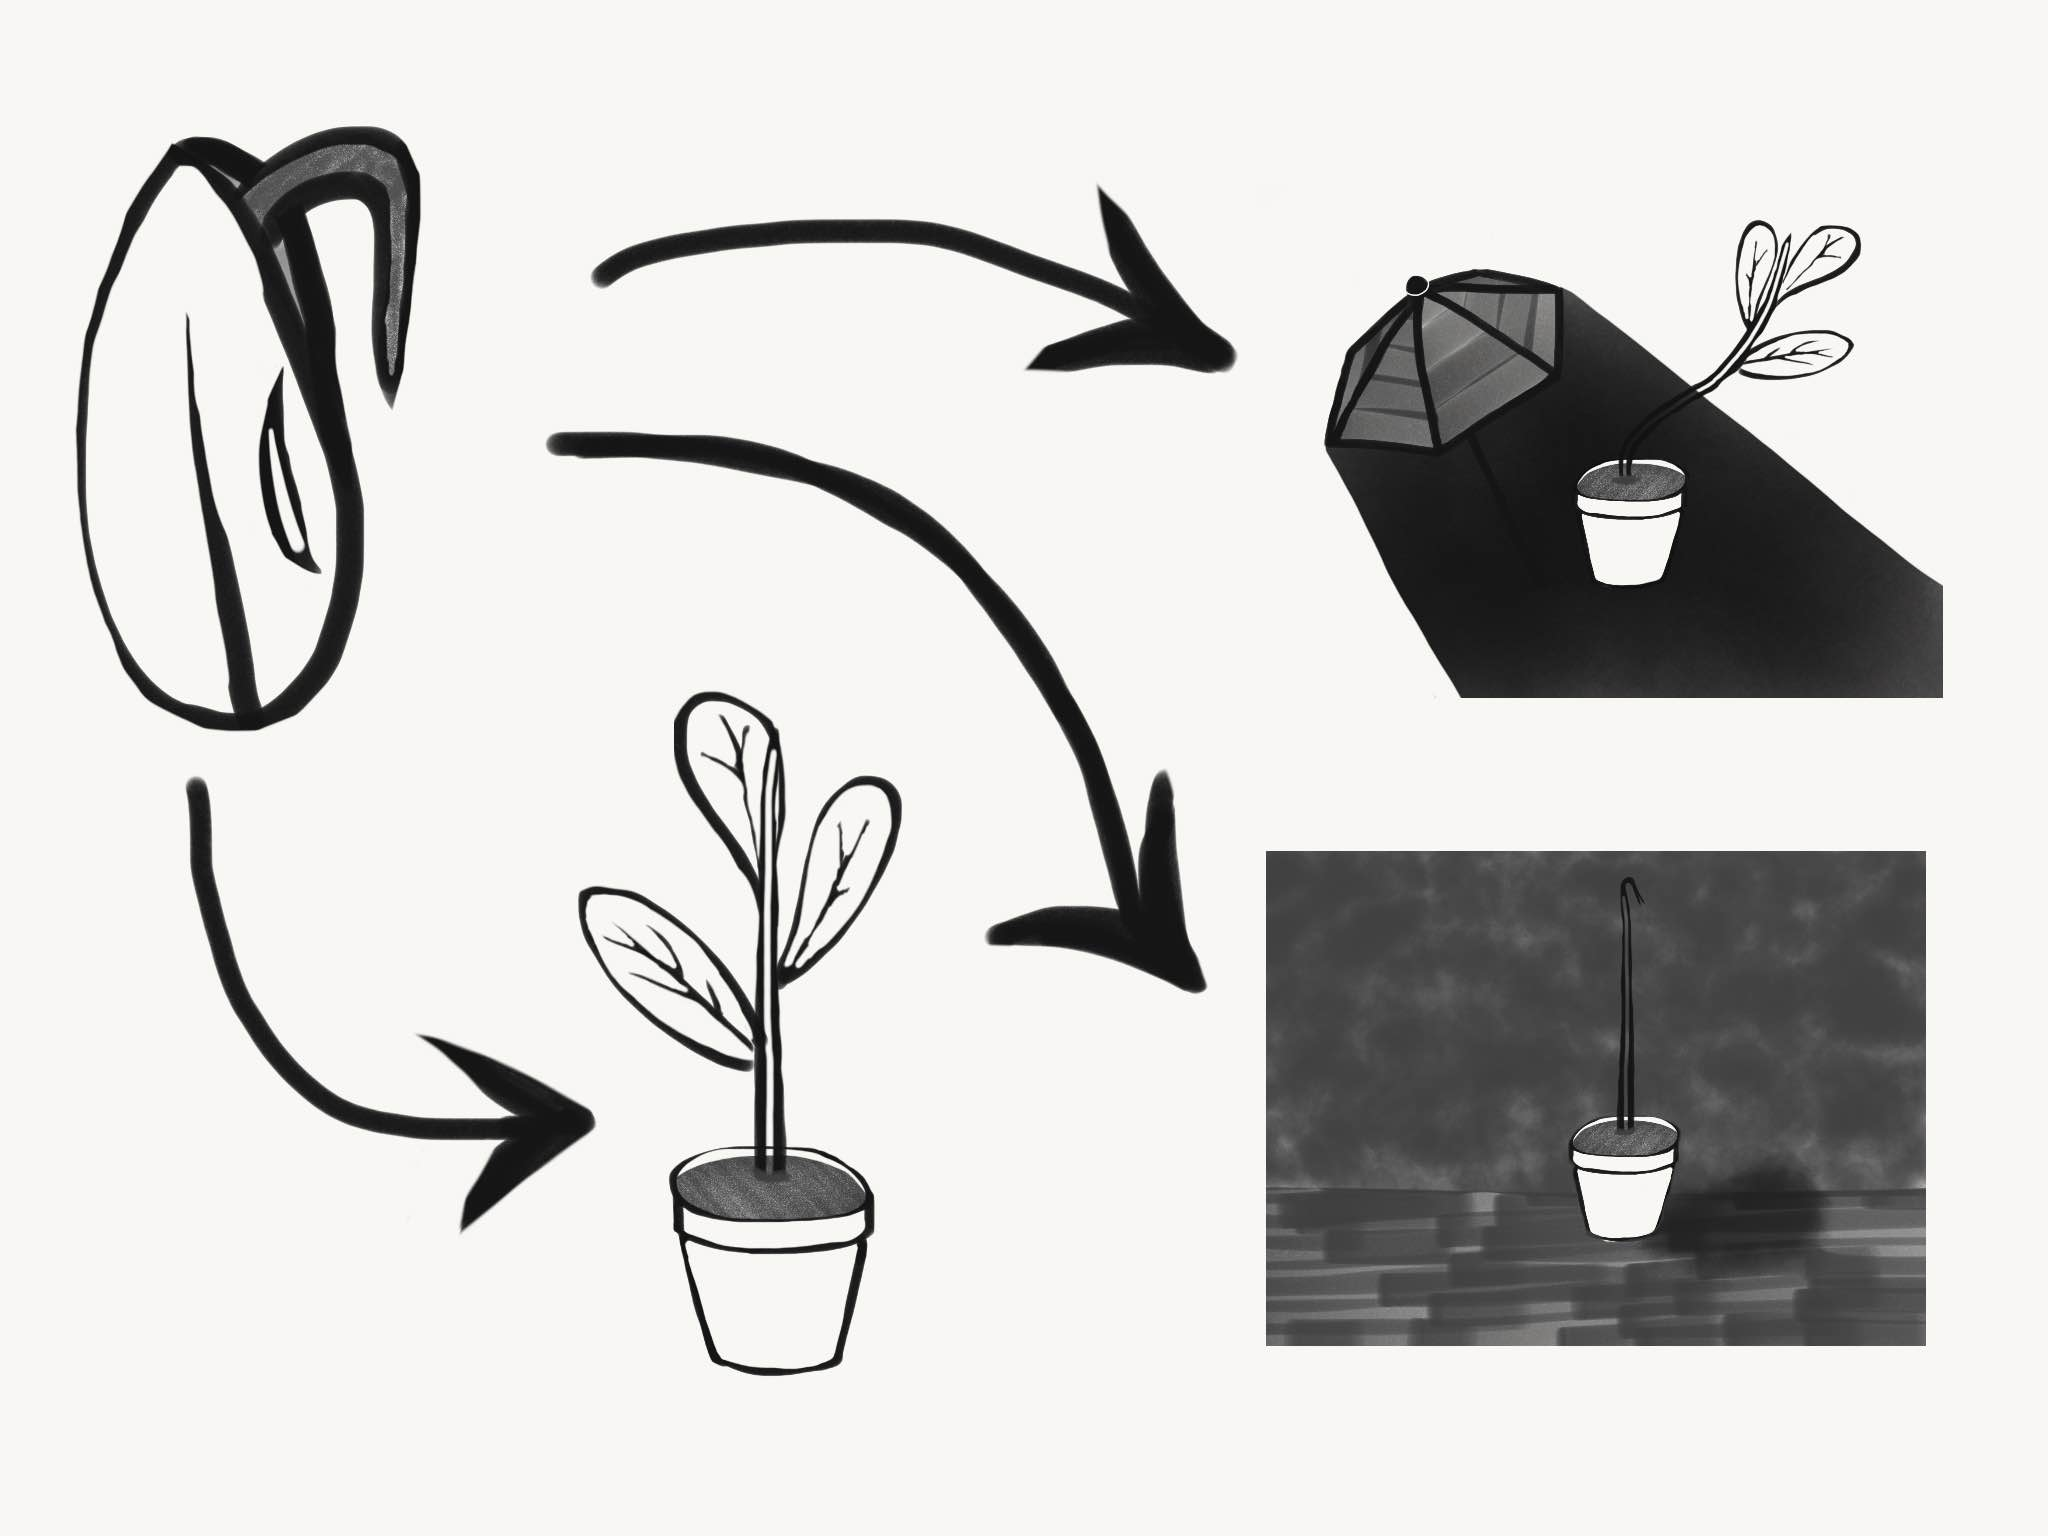
\includegraphics[width=0.8\textwidth]{img/plant_developmental_perturbation.jpg}
  \captionsetup{singlelinecheck=off,justification=raggedright}
  \caption{A cartoon illustration of alternate phenotypes expressed based on environmental signals.}
\end{figure}

\end{frame}

\begin{frame}{Indirect Plasticity: Conditional Initial State}
\begin{figure}
  \centering
  \begin{subfigure}[b]{0.5\textwidth}
    \centering
    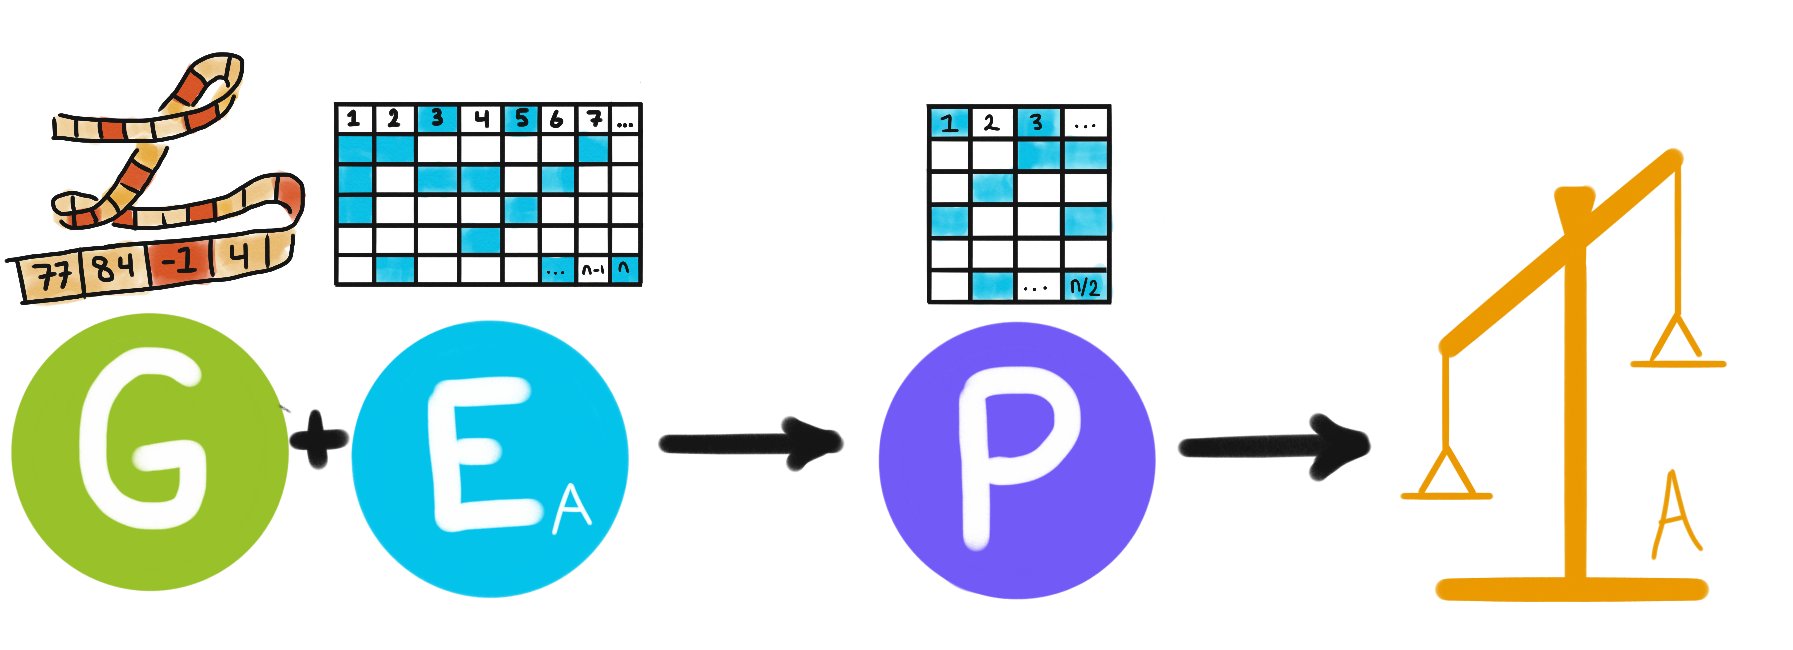
\includegraphics[width=\textwidth]{img/indirectschemeA} \\
    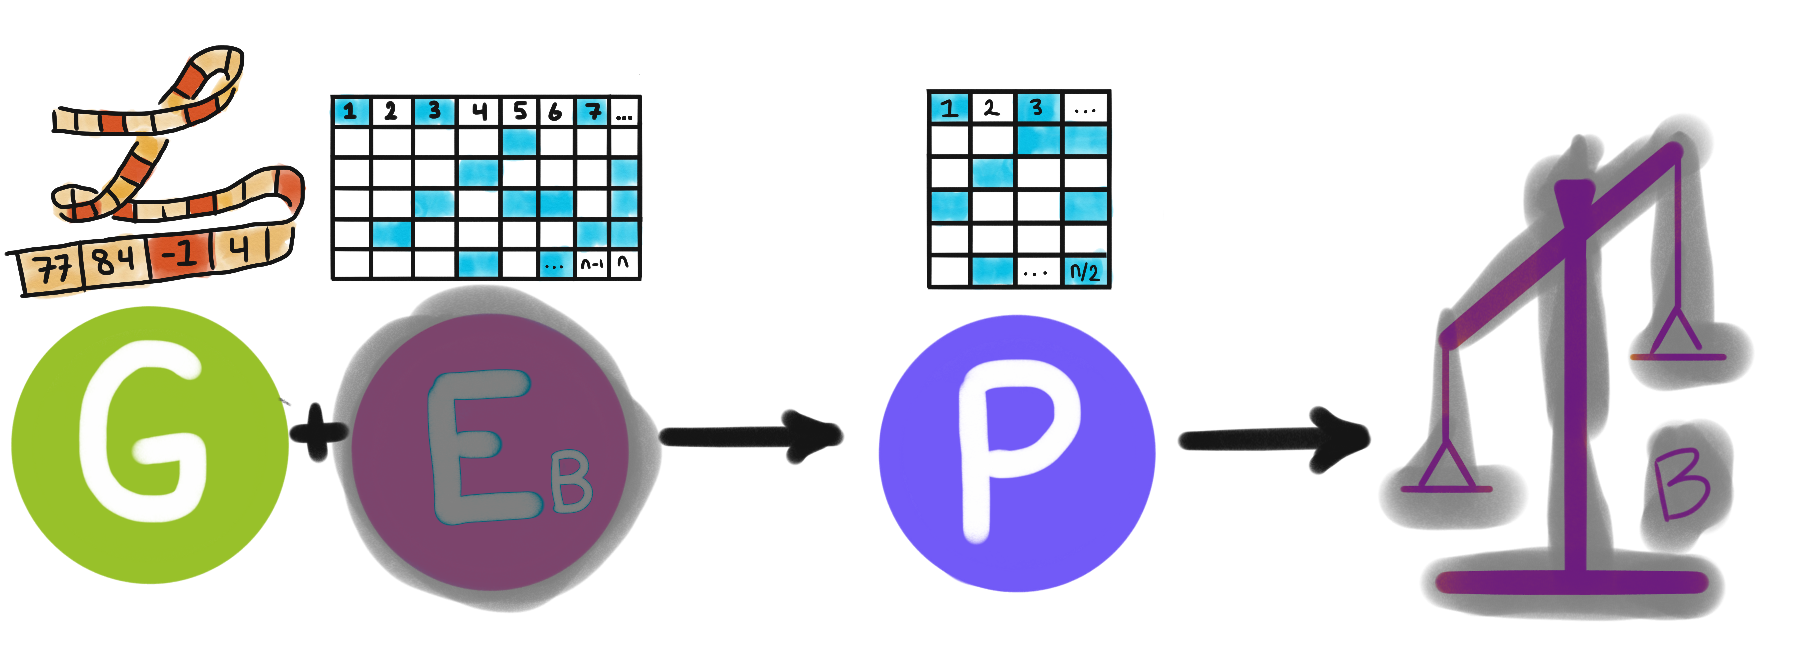
\includegraphics[width=\textwidth]{img/indirectschemeB}
    \caption{experimental scheme}
    \label{subfig:directscheme}
  \end{subfigure}%
  \hfill
  \begin{subfigure}[b]{0.5\textwidth}
    \centering
    
 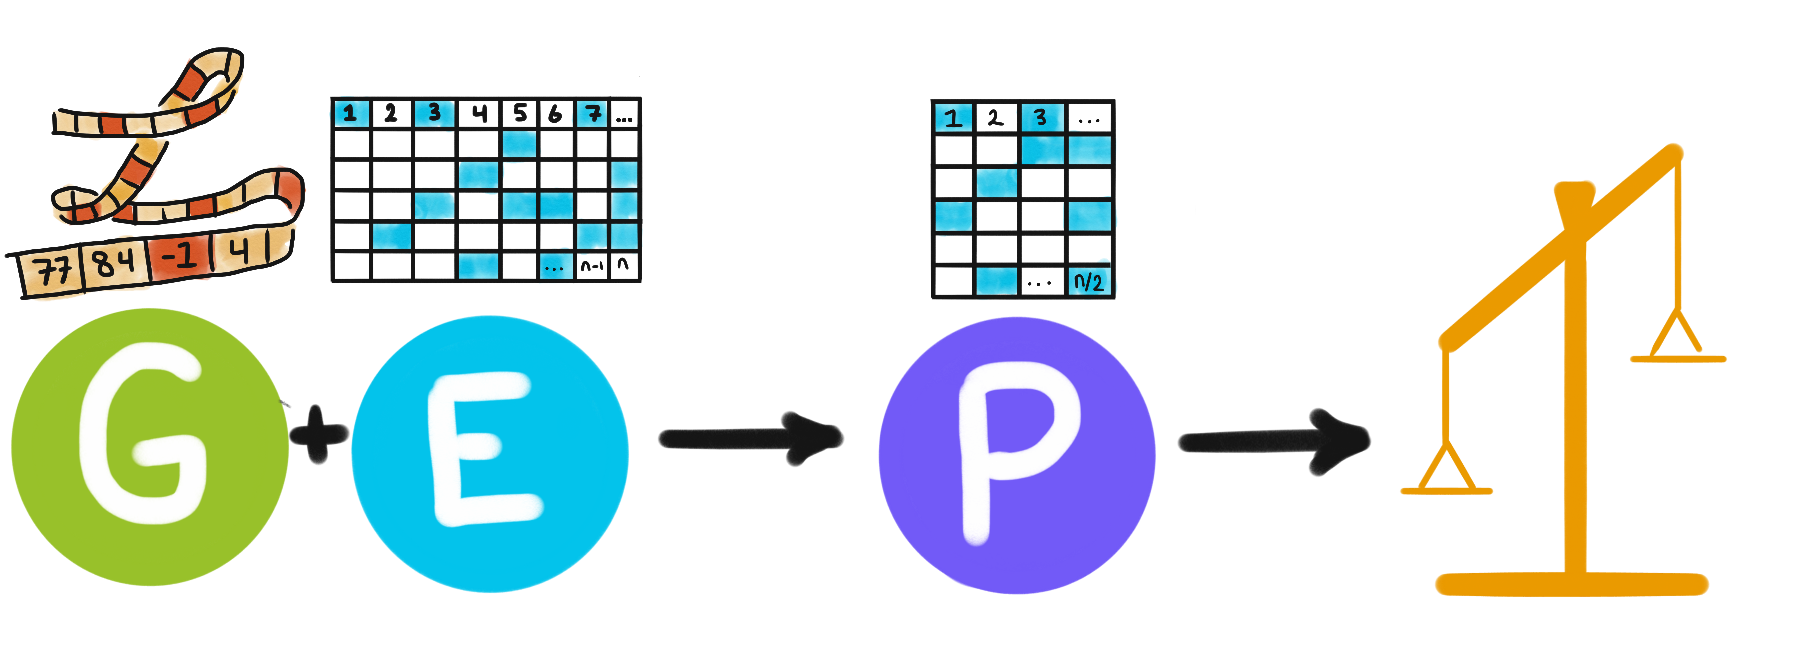
\includegraphics[width=\textwidth]{img/modelscheme} \\
 \vspace{5ex}
    
    \caption{control scheme}
     \label{subfig:controlscheme}
  \end{subfigure}
  \captionsetup{singlelinecheck=off,justification=raggedright}
  \caption{A comparison of the control and experimental schemes employed to investigate the relationship between indirect plasticity and evolvability.}
  \label{fig:direct_plasticity_scheme}
\end{figure}
\end{frame}

\begin{frame}{Mutational Outcome Frequencies}
\begin{figure}
    \centering
    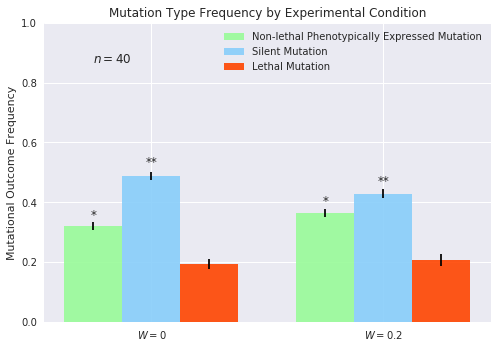
\includegraphics[width=0.8\textwidth]{img/mutation_type_indirect}
 	\captionsetup{singlelinecheck=off,justification=raggedright}
  	\caption{Comparison of mutational outcome frequencies for champions evolved with only primary condition/objective pair versus with both primary and secondary condition/objective pairs.}
    \label{fig:mutation_type_indirect}
\end{figure}
\end{frame}


% \begin{frame}{Indirect Plasticity Results: Summary}
% \begin{itemize}
%   \item indirect plasticity observed
%   \item indirect plasticity increases sensitivity to mutation
% \end{itemize}
% \end{frame}